\documentclass{article}
\usepackage[utf8]{inputenc}
\usepackage{graphicx}
\begin{document}
\section{ Processamento de linguagens }

\subsection{ Título nível 2 }

\subsubsection{ Título nível 3 }


Isto é um \textit{ ficheiro } de \textbf{ teste }
Exemplos:

	- \textit{ Italico } -> começa por \%
	- \textbf{ Negrito } -> começa por \$

\section{ \textit{ Itálico dentro de um título } }


Lista:

\begin{itemize}
 
	
	\item  elemento 1
	
	\item  elemento 2
	
	\item  elemento 3
	
	\item  \textbf{ elemento a negrito na lista }
\end{itemize}

	- elemento fora do contexto de lista
	
\begin{figure}[h]
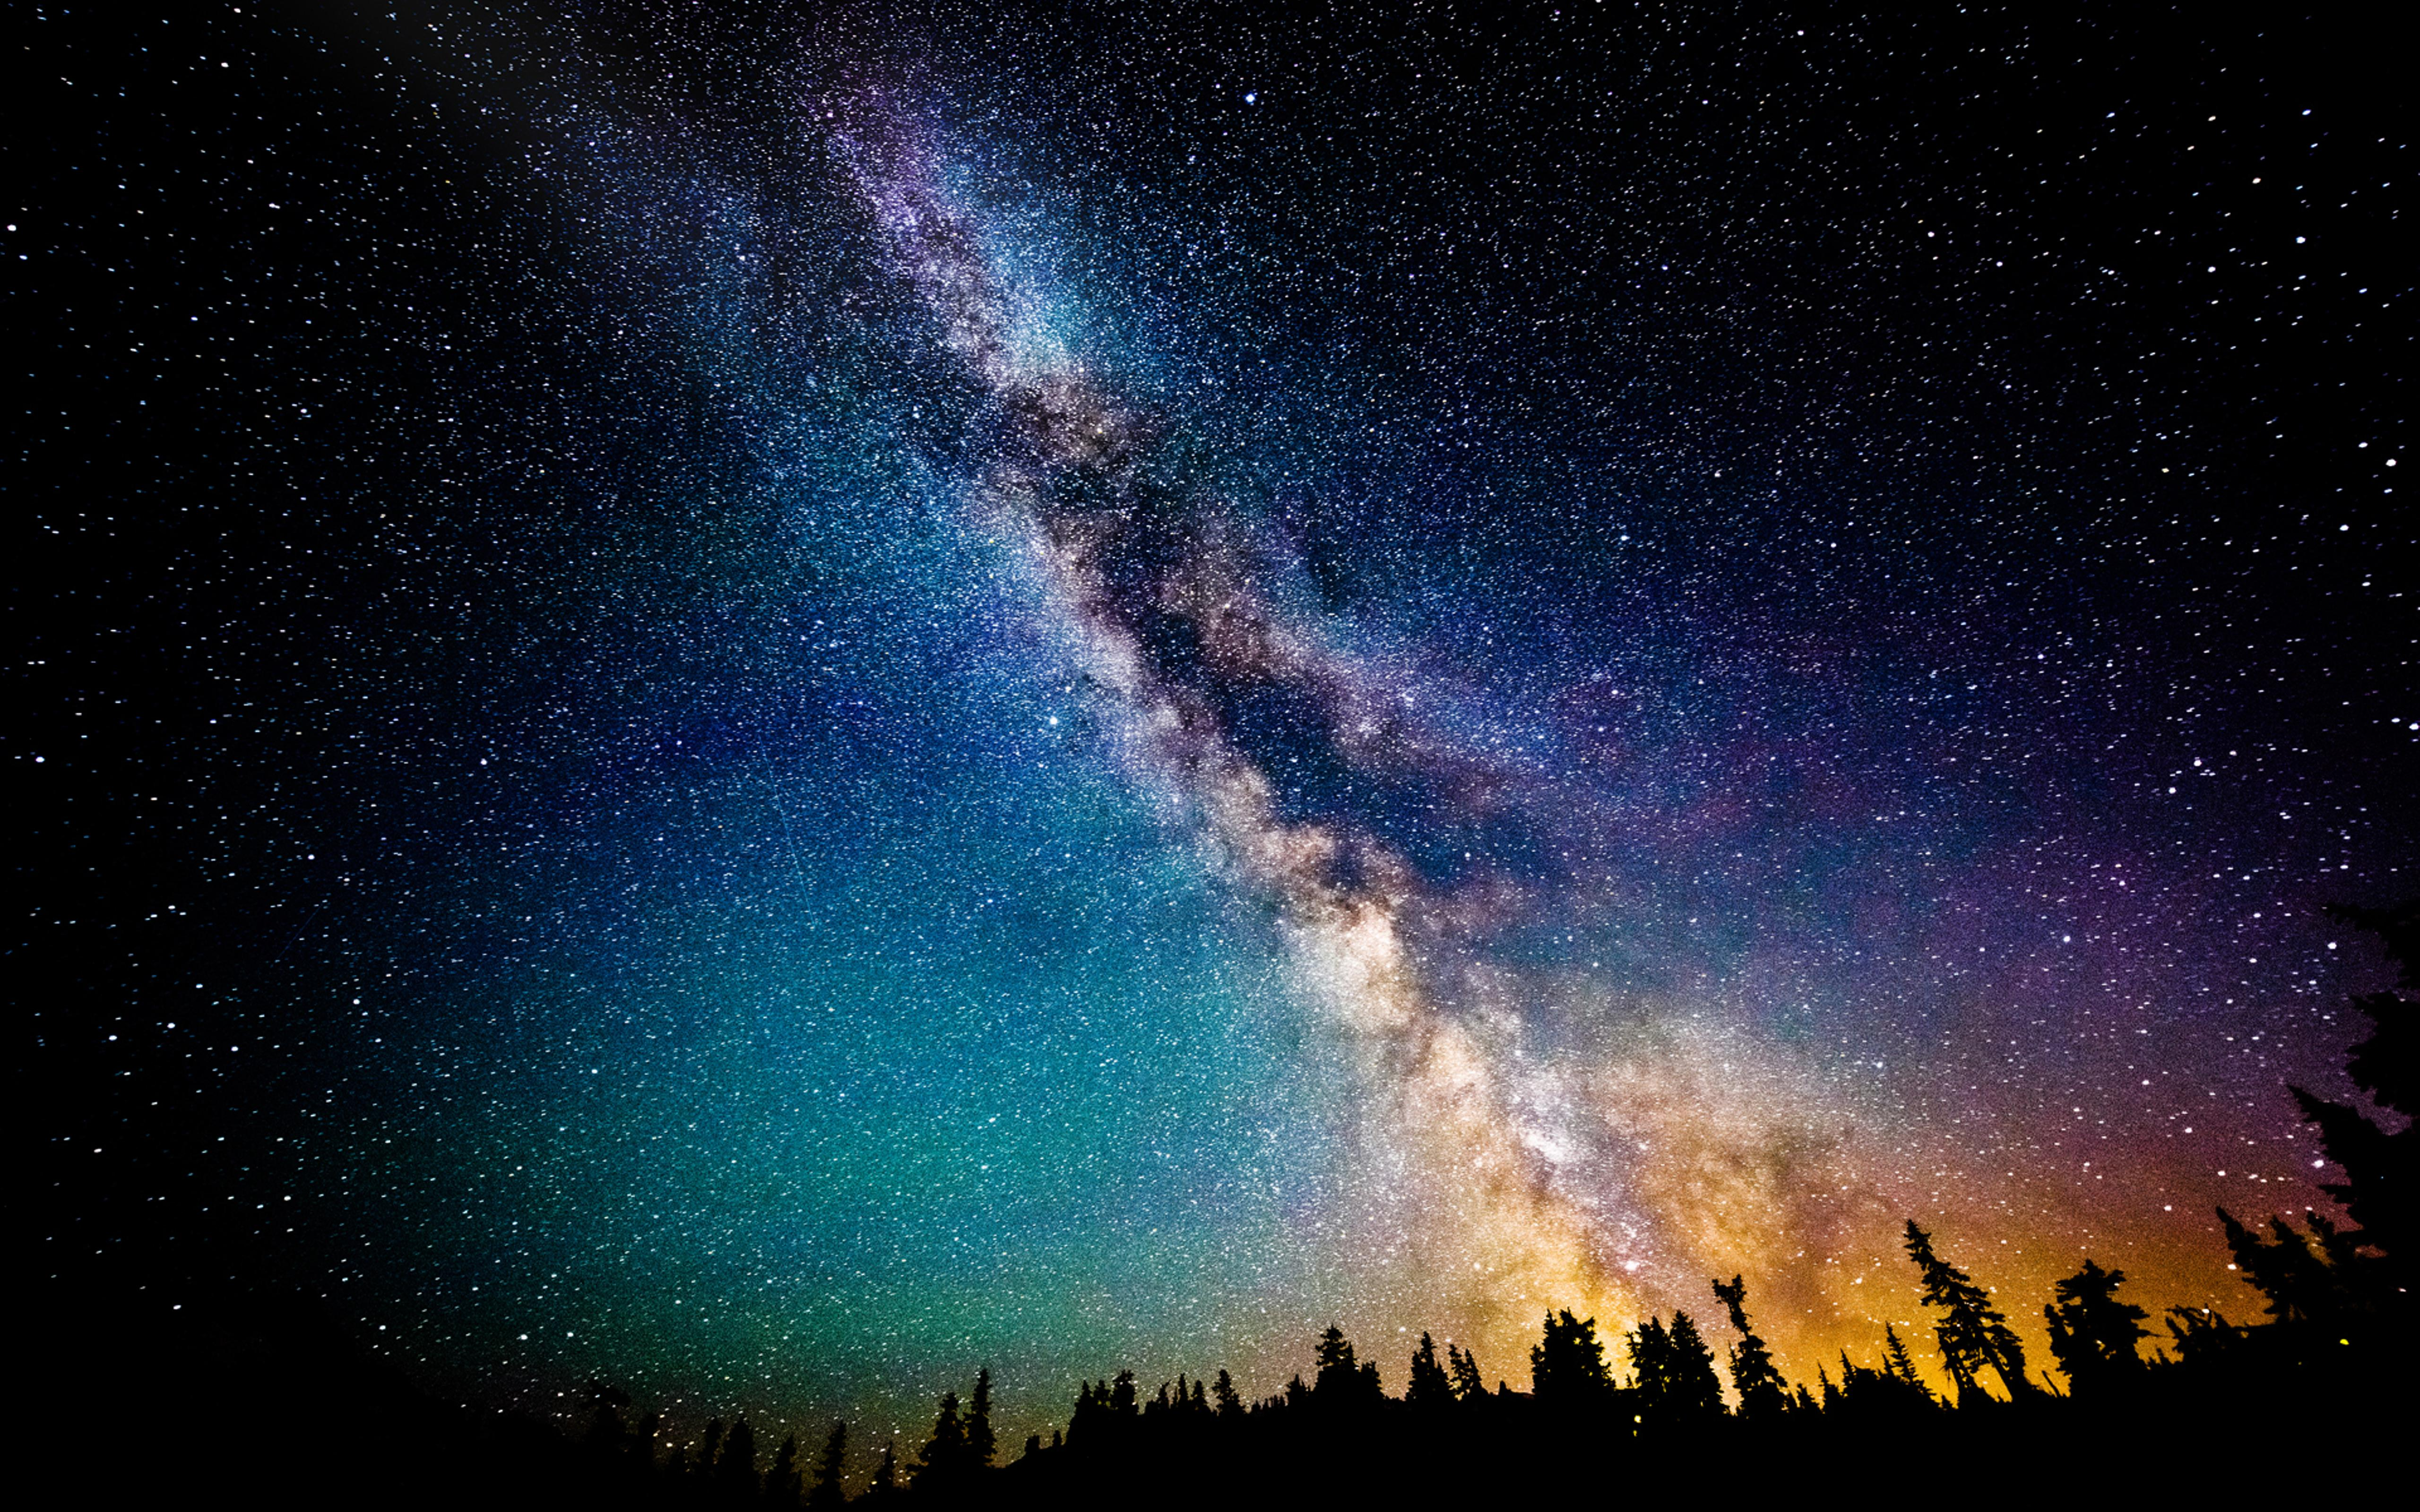
\includegraphics[width=400px]{ Image1.jpg }

\end{figure}


\begin{figure}[h]
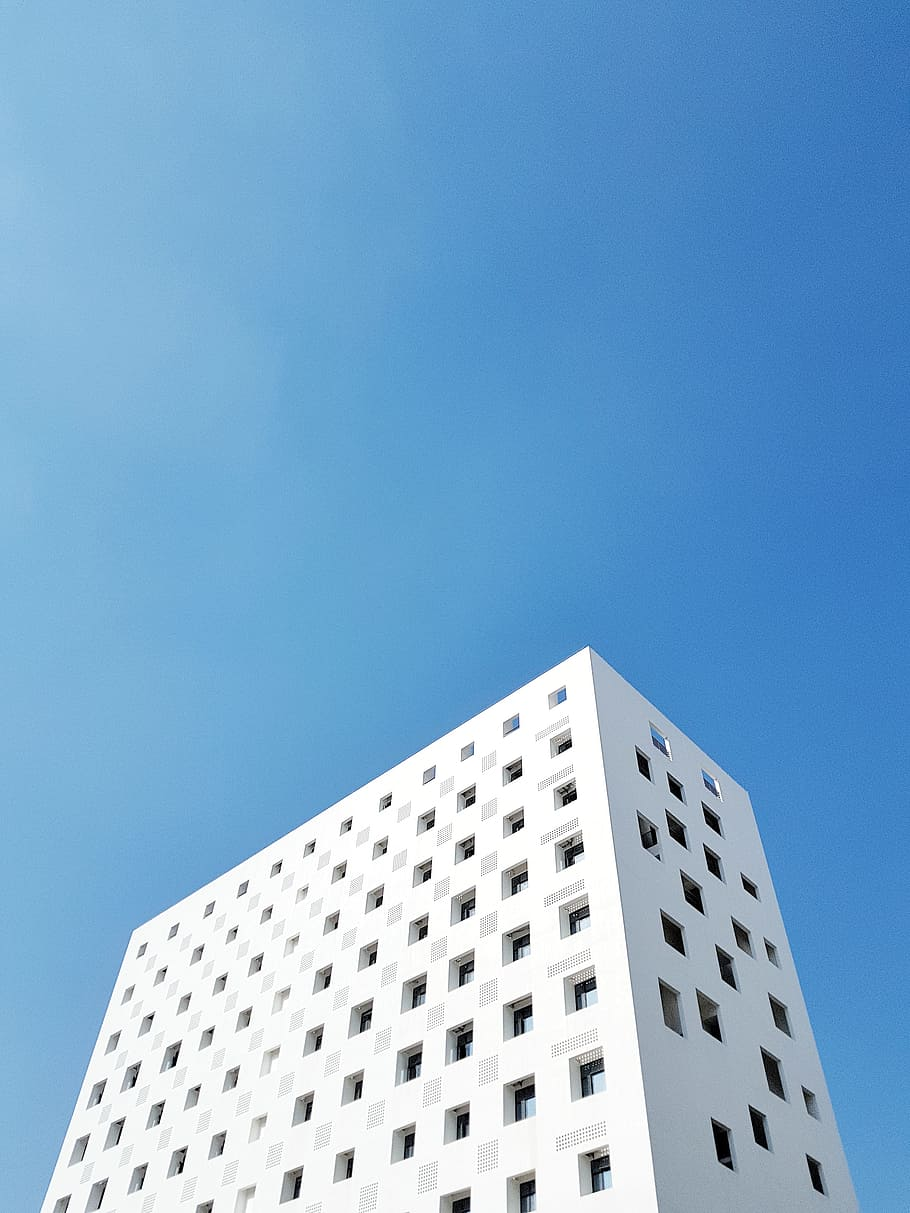
\includegraphics[width=400px]{ Image2.jpg }
\caption{ Legenda da imagem 2 } 
\end{figure}


\begin{figure}[h]

\includegraphics[width=400px]{ Image3.jpg }
\caption{ Legenda da imagem 3 com \textit{ italico } e \textbf{ negrito } e caracteres especiais \% \$ } 
\end{figure}

\end{document}
